	\section{Experimental Evaluation}
	
	We implemented our code in Python 3.8.
	Gurobi 9.52 was used for solving the MILP problems. We conducted our evaluation on an AMD Threadripper 7970X ($32$ cores$@4.0$GHz) with 256 GB of main memory and 2 NVIDIA RTX 4090. 
	
	We consider two DNNs: one for MNIST, namely a pre-trained $5\times 100$ (available at \url{https://github.com/eth-sri/eran}), a 5 fully connected layers DNN, with 100 neurons each,	trained with diff AI \cite{deeppoly}. 
	Although it is relatively small, it is also of good quality with $97\%$ accuracy on classification, but it is not easy to certify for global robustness (the size of a network can be deceptive to know whether they are easy or hard to verify \cite{ATVA25}).  
	The second one is a 2 fully connected layers, 50 neurons each, learnt as a surrogate model, with 10 reduced input and 10 reduced output, that predict the plastic strain in 3000 points of a mesh over a pipe given the deformation of each of this 3000 points (through a PCA order reduction encoding all 3000 points with 10 dimensions in input and 26 dimensions in output), from \cite{aiware}.
	
	MNIST is a classification benchmark, we thus report different bound $\beta^{\epsilon}_{i,j}$
	for an $L_1$-deformation $\leq .5$. The pipe considers a conjunction of $L_1 \leq 3.9$ and $L_\infty \leq 0.2$ perturbations, corresponding to physically pertinent dimensions, and 
	maximizes the sum of the difference in output of 10 selected points in the mesh between an input and its deformation.

For each benchmark, we report three value: the bound obtained (lower value is better),
the solution obtained (distance to the bound depicts how close the model has converged),
and worst-case (higher is better) which is taking the solution as input to the DNN. For a fully accurate model ("2v" or classical and all variables binary),
the worst-case will equal the solution, otherwise, it will be smaller due to abstraction.

\subsection{Classical vs our "2v" model}

We start by evaluating how accurate the 2v model is vs the classical encoding, both when half the ReLUs are approximated with the LP relaxation, and when all the ReLUs are encoded exactly. We use the pipe models which is easier to verify, and set the time-out at 1000s for both models.

\begin{table}[h!]
	\begin{tabular}{|l|c|c|c|}\hline\hline
		model &        Bound $\downarrow$ &  Sol. &      Worst-Case $\uparrow$ \\\hline \hline
	Classical, $50 \times 2$ &    $.320$ &  $.320$ & $.017$ 
    \\\hline
    2v model, $50 \times 2$ &    {\bf .040} &  $.037$ & {\bf .018} 
    \\\hline \hline
    Classical, $100 \times 2$ &  .186  &  $.022$ & $.022$ 
    \\\hline
	2v model, $100 \times 2$&     {\bf .042} &  $.023$ &   {\bf .023} 
    \\\hline \hline
	\end{tabular}
	\caption{Comparison of the classical encoding with our "2v" model on the pipe system with a fixed timeout of 1000s, with either $50 \times 2$, 
    or the full $100 \times 2$ binary variables.}
    \label{table.classical}
\end{table}

We confirm that the LP relaxation of the classical model is extremely poor, with bounds $8$ times worse than using our "2v" model. Further, even using a fully accurate model with all $100 \times 2$ variables encoded as binary variables, the "2v" model produces bounds $>4$ times better than the classical model, due to the internal Branch and Bound process to compute bounds, which uses linear relaxation.

	\subsection{Experimental results for robustness (MNIST)}
	

	
	\begin{table}[h!]
	\begin{tabular}{|l|c|c|c|c|}\hline\hline
		model &        Bound$\downarrow$ &  Sol. &      Worst-Case$\uparrow$ &  Time(s) \\\hline \hline
		1v, $375 \times 1$ & 17.472 & .909 & .092 & 43200 \\\hline 
		2v, $375 \times 2$ & 21.013 & 8.467& .223 & 43200 \\\hline		
		2v, $450 \times 2$ & 12.010 & 3.441 & {\bf .258} & 43200 \\\hline
		1v, $500 \times 1$ & ?? & ?? & ?? & 43200 \\\hline 
		3v, $500 \times 3$ & ?? & ?? & ?? & 43200 \\\hline 
	 2v, $500 \times 2$ & {\bf 8.761} & nan & nan & 43200 \\\hline\hline

	 2v, $485 \times 2$ & 20.646 & 1.915 & {\bf .372} & 130000 \\\hline\hline

		 2v, $500 \times 2$ & {\bf 8.257} & nan & nan & 260000 \\\hline\hline
		 
	\end{tabular}
	\caption{Comparison of "1v", "3v" and "2v" models 
	to obtain bounds on $\beta^{.5}_{6,8}$ on the {\bf full dimension} MNIST DNN, for timeouts of 43200s, 130000s and 260000s, where 375, 450, 485 or 500 ($\times 1$, $\times 2$, $\times 3$) neurons use binary variables.}
\end{table}

On the full space, we reach bounds of $8.2$ (on $\beta^{.5}_{6,8}$), which is too pessimistic as it allows to certify 0 image robust. The worst-case found by the "2v" $485 \times 2$ binary variables after 130000s only displays a difference of 
$0.37$, $20 \times$ away from the bound found.

\begin{figure*}[t!]
	\centering

\includegraphics[scale=0.5]{image.png} \hspace{0.8cm}
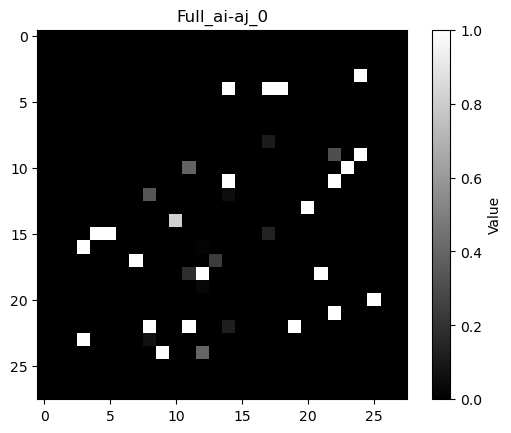
\includegraphics[scale=0.5]{perturb.png}
\caption{An improbable image and its perturbation (difference at x=13, y=18) 
with maximal $\beta^{.5}_{6,8}=0.37$ for MNIST as obtained by the "2v" $485 \times 2$ model in full 784 dimension image space.}
\end{figure*}	




\paragraph{Reduced space}

We now consider a PCA model order reduction to avoid considering improbable images, 
speed up obtaining the bounds, and obtain less pessimistic bounds.
We settle on 20 orders, as the MNIST DNN considered run on a images obtained from projecting to the reduced order and projected back to the full dimension 
display the same accuracy of $97$\% as the DNN on the original images, meaning no accuracy is lost from reducing to 20 dimensions, which is the only thing which matters. On such a reduced space, bounds obtained are much more precise, and one can certify robustness of images online.



	\begin{table}[h!]
	\begin{tabular}{||l||c|c|c||}\hline\hline
		model &        Bound$\downarrow$ &  Sol. &      Worst-Case$\uparrow$ \\\hline \hline
1v, $400 \times 1$ & $1.414$ &  $.691$ & $.010$ \\\hline 
3v, $400 \times 3$ & $1.186$ & $.600$ & $.003$ \\\hline 
2v, $400 \times 2$ & $1.274$ & $.566$ & $.002$ \\\hline\hline
	 
1v, $475 \times 1$ &  $1.408$ & $.301$ & $.008$  \\\hline 
3v, $475 \times 3$ &  $1.153$ & $.250$ & $.006$ \\ \hline 
2v, $475 \times 2$ &  $1.247$ & $.1957$ & $.019$ \\\hline\hline


1v, $500 \times 1$ & $1.412$ & $.161$ & .057 \\\hline 
3v, $500 \times 3$ & {\bf 1.137} & $.103$ & $.065$\\\hline 
2v, $500 \times 2$ &  $1.182$ & $.084$& {\bf .084}  \\\hline\hline
	 
	\end{tabular}
	\caption{Comparison of "1v", "3v" and "2v" models 
	to obtain bounds on $\beta^{.5}_{6,8}$ on the {\bf 20 dimension}  reduced order MNIST DNN, for timeouts of 14400s, where 400, 475,  or 500 ($\times 1$, $\times 2$, $\times 3$) neurons use binary variables.}
\end{table}






\begin{figure*}[t!]
	\centering
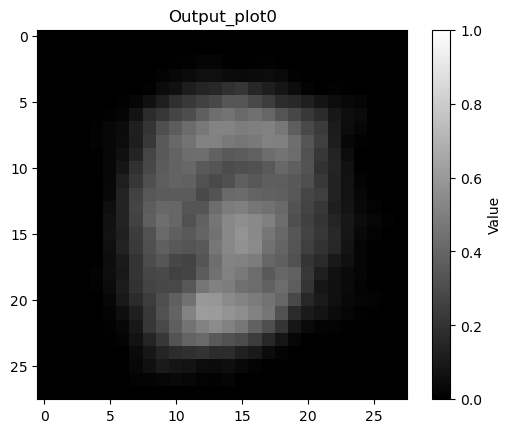
\includegraphics[scale=0.5]{redimage.png} \hspace{0.8cm}

\includegraphics[scale=0.5]{redperturb.png}
\caption{An image and its perturbation from the 20-dimension reduced space with maximal $\beta^{.5}_{6,8}=.084$ for MNIST as obtained by the "2v" $500 \times 2$ model.}
\end{figure*}	

	
	
\begin{table}[h!]
	\begin{tabular}{||l||c|c|c|c||}\hline\hline
		model &    $L_1\leq 0.5$ & $L_1\leq 1$ & $L_1\leq 1.5$ &  $L_1\leq 2$ \\\hline \hline
		1v, $500\times1$ & $80 \%$ & $32\%$ & $7\%$ & $0\%$ \\\hline
		3v, $500 \times 3$ & {\bf 86 \%} & {\bf 53\%} & {\bf 20\%} & {\bf 4\%} \\\hline
		2v, $500 \times 2$ & 84\% & 51\% & 16\% & {\bf 4\%} \\\hline \hline
	\end{tabular}
	\caption{Comparison of "1v", "3v" and "2v" models 
	in the percentage of images they can certify in real-time for different values of $L_1$-perturbations.}
    \label{table.cert}
\end{table}


	


\subsection{Experiment results for regression (Pipe strain)}
	
	For the pipe system, to find a example of large difference on outputs is one of the main aims.

	\begin{figure*}[t!]
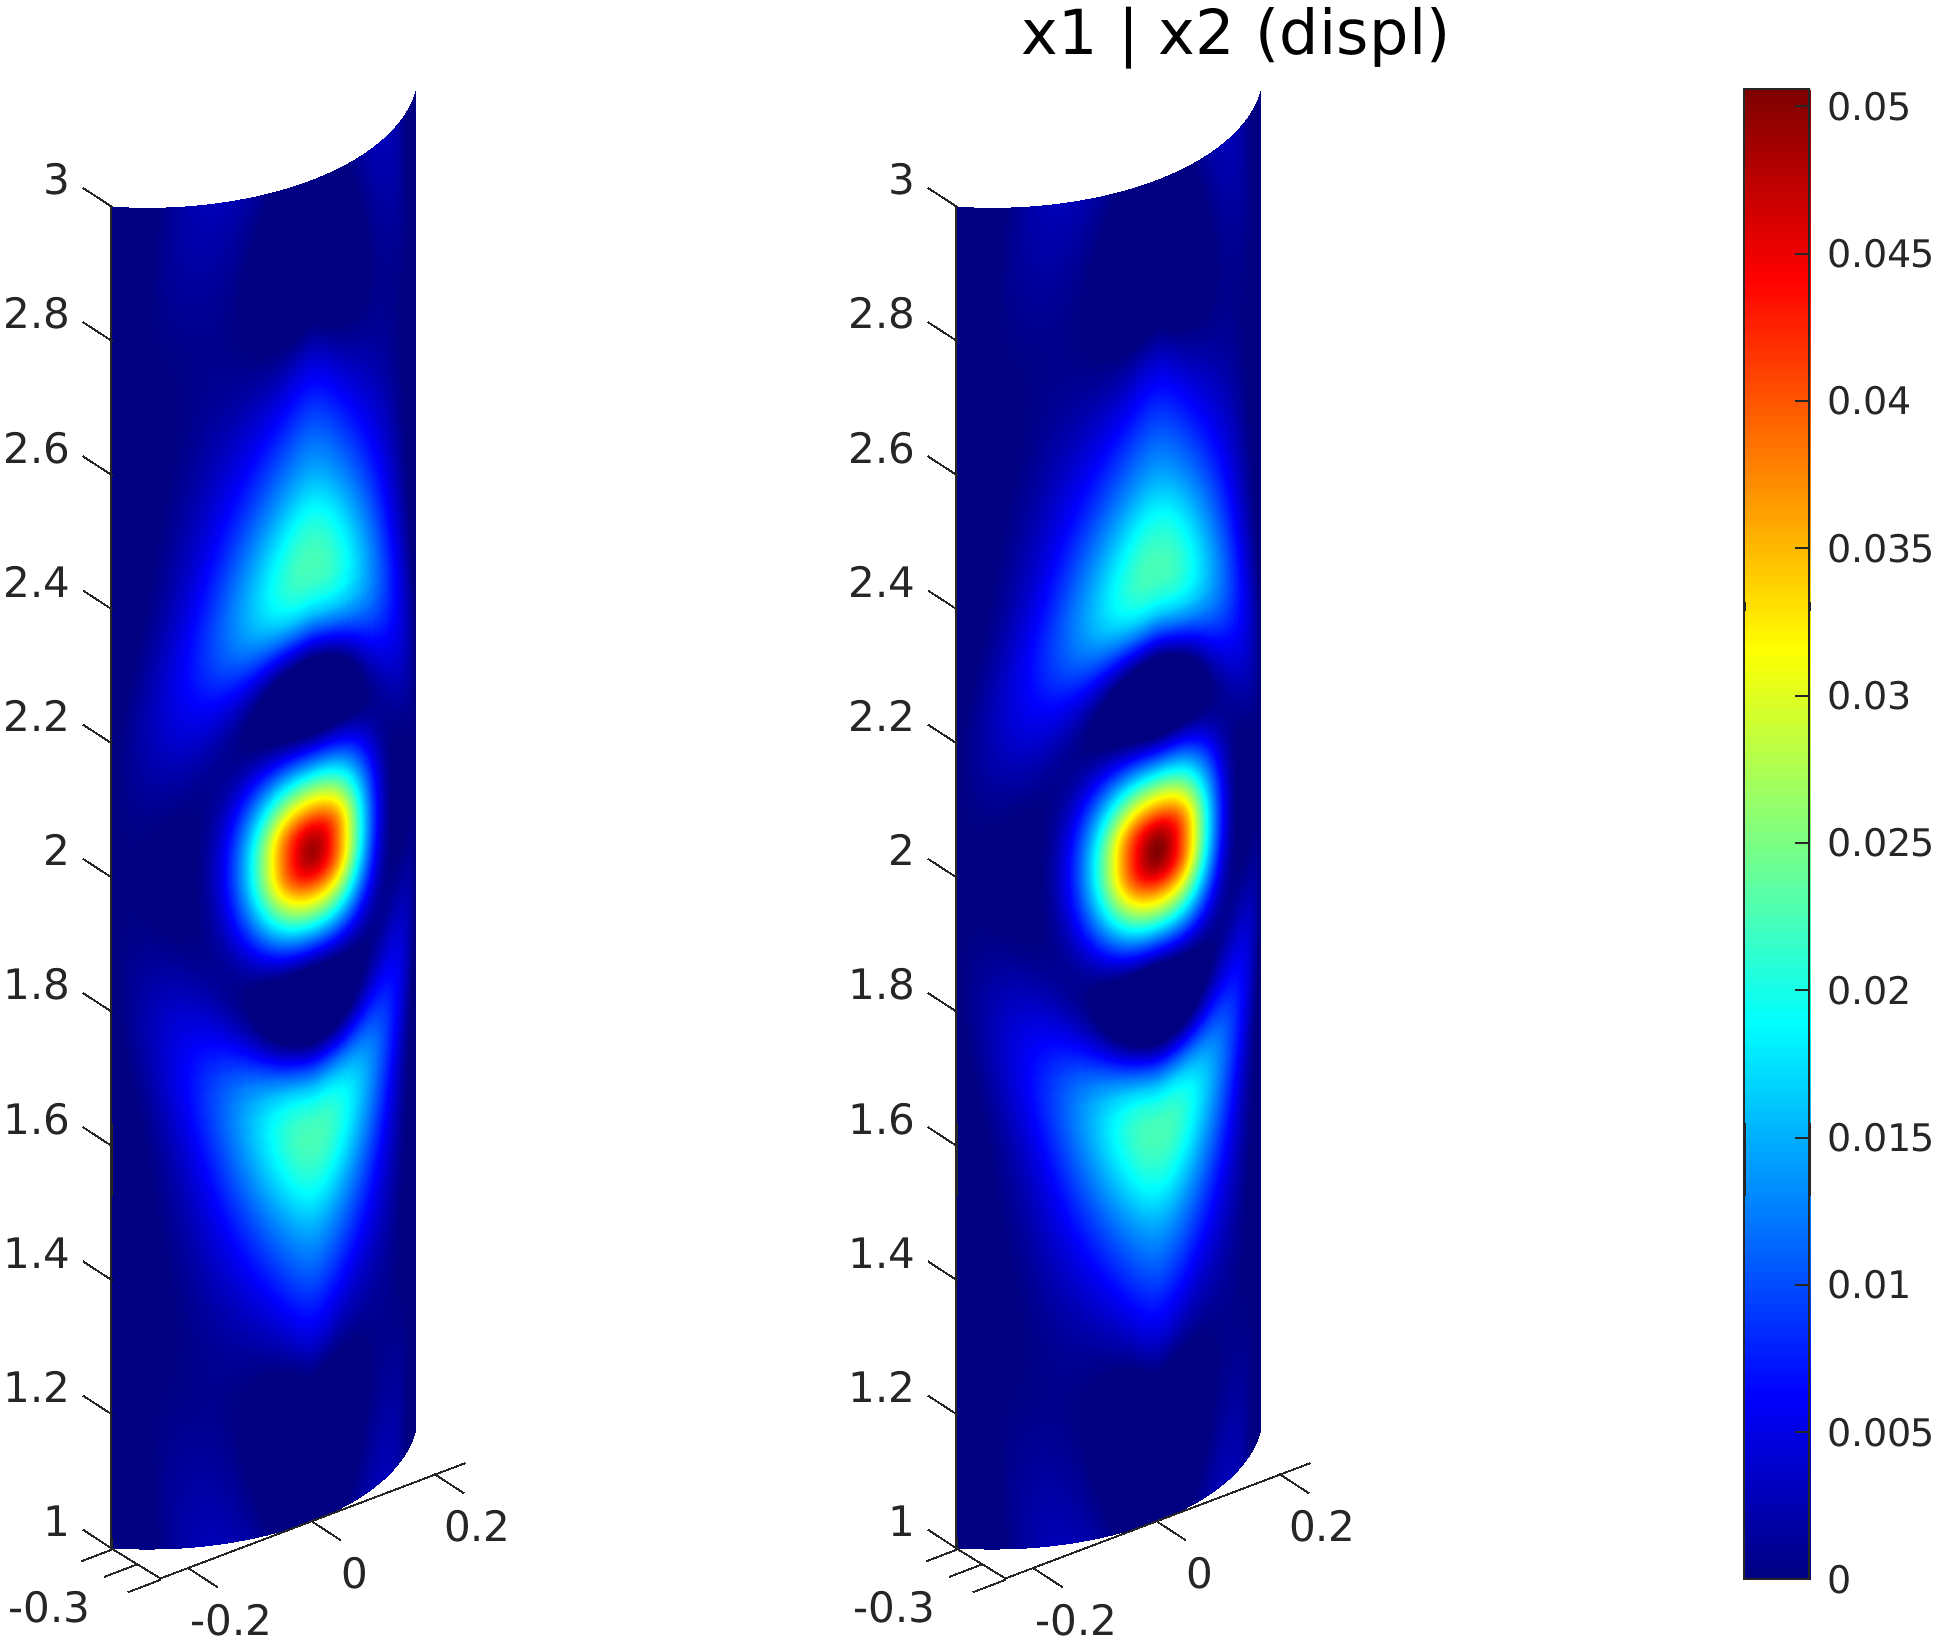
\includegraphics[scale=0.5]{deform.png} \hspace{0.8cm}
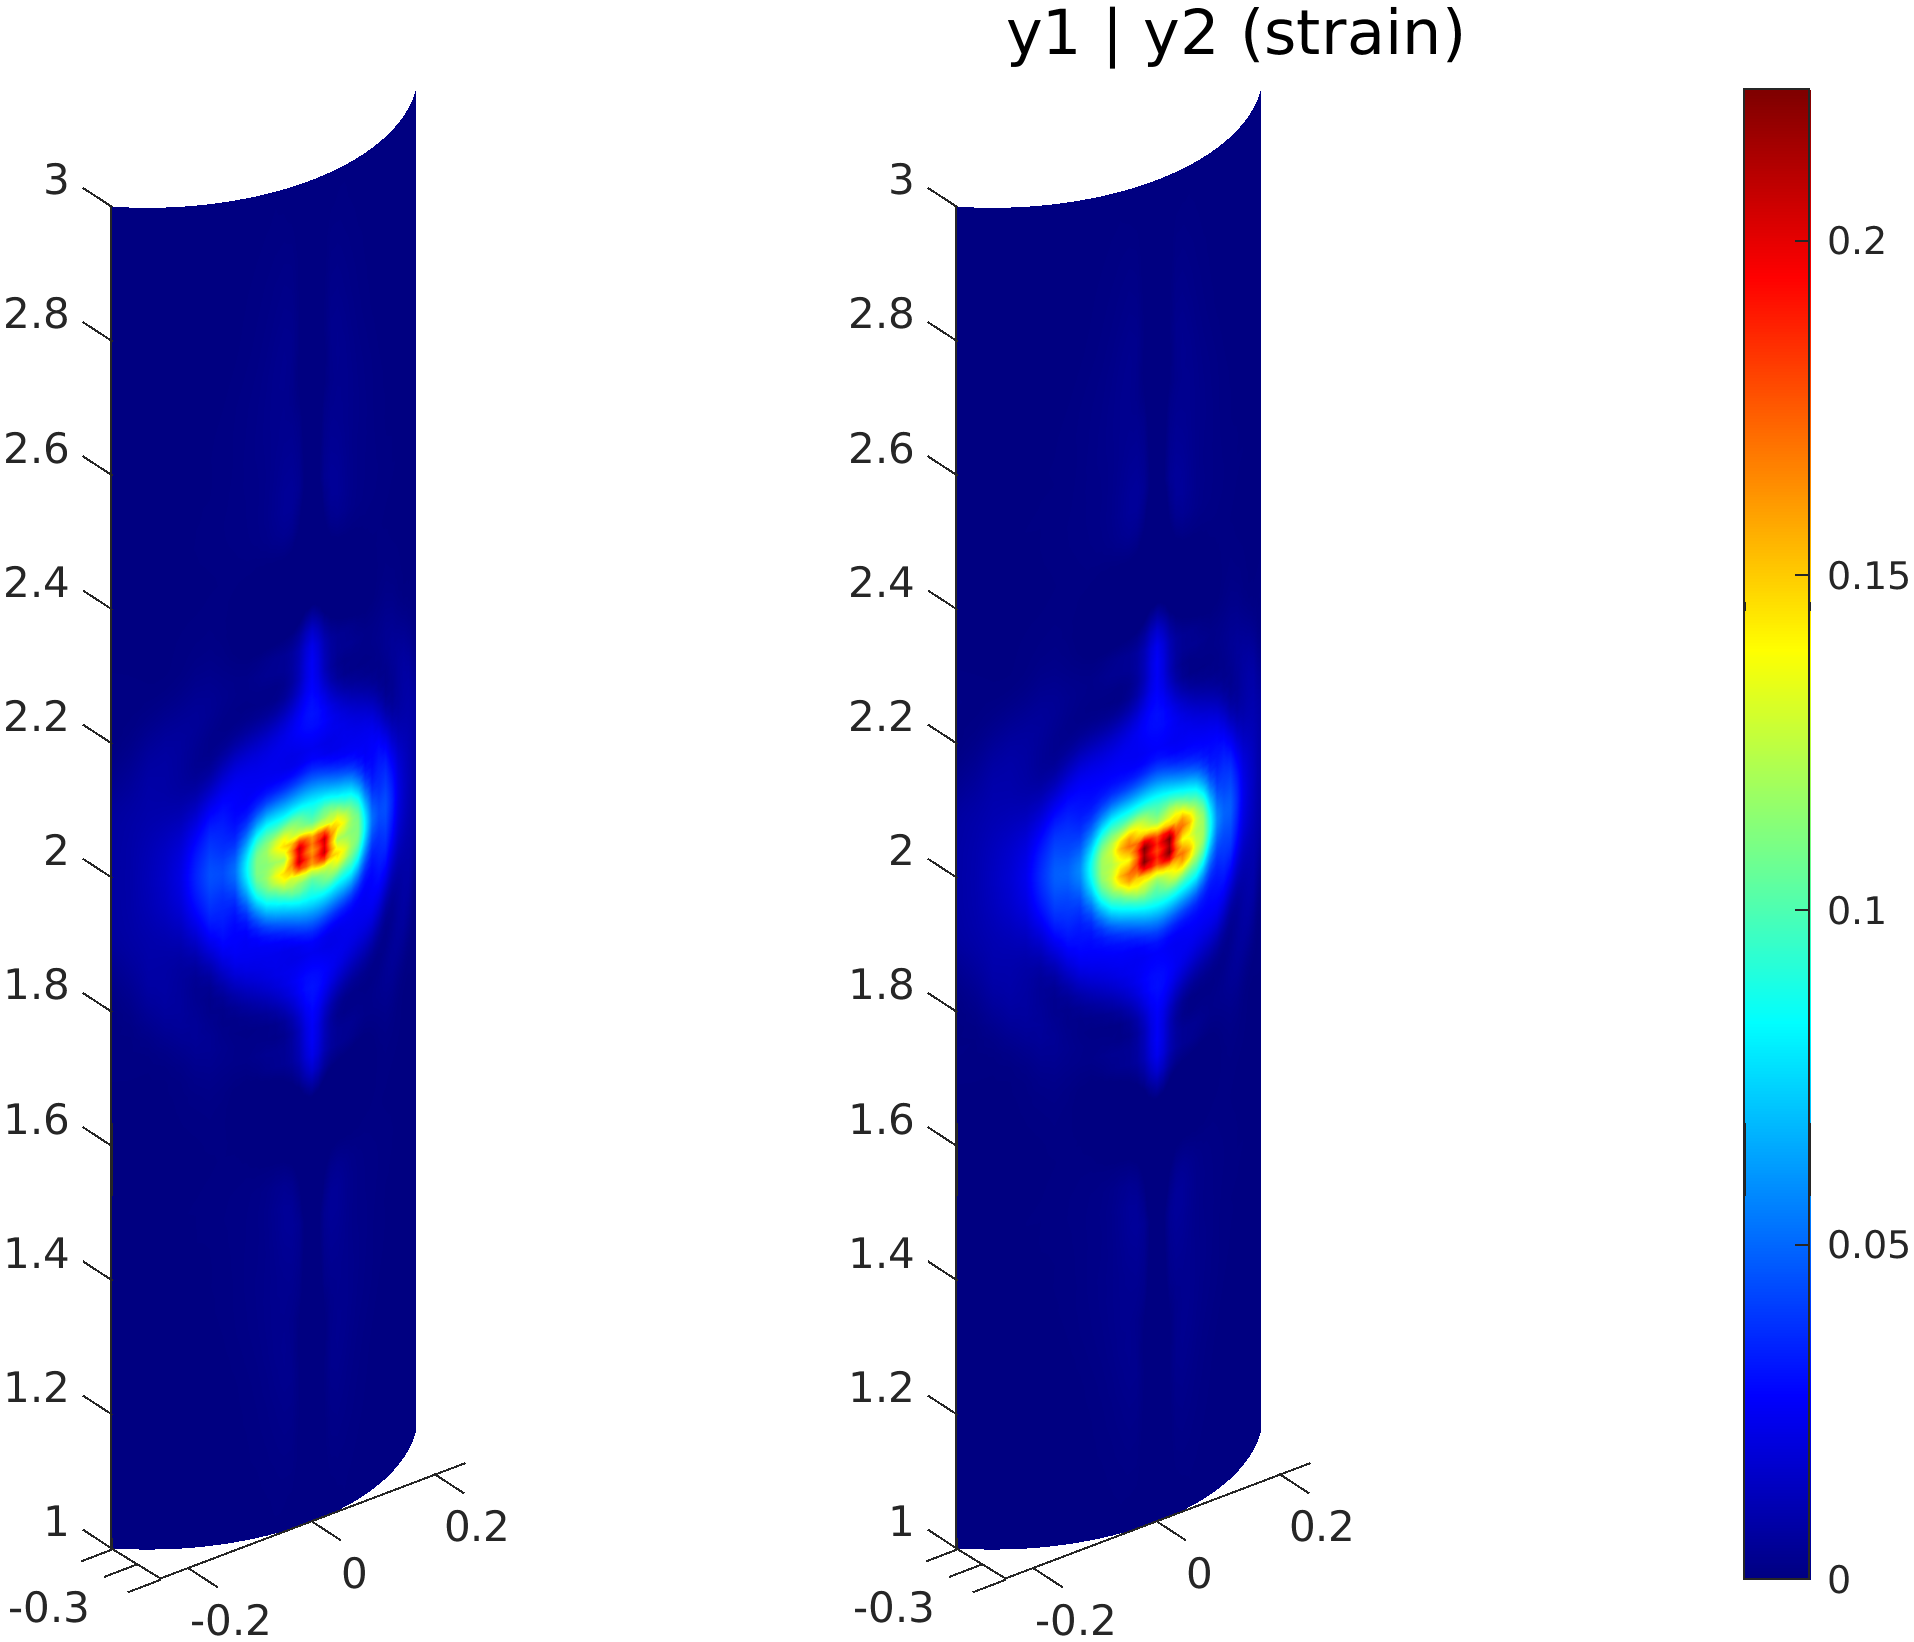
\includegraphics[scale=0.5]{strain.png}
\caption{2 slightly different deformations and their associated quite different strain as obtained by the "2v" $100 \times 2$ model.}
\end{figure*}	


	The network of Pipe system is relatively simple and in the tests, we will open all $\ReLU$ nodes.

	

	We will compare the results of different modeling methods.
	
	\vspace*{1ex}
	
	\iffalse
	\begin{table}[h!]
	\begin{tabular}{|l|l|l|l|l|}\hline
		$L_1\leq 0.83$ &        Bound $\downarrow$ &  Solution $\uparrow$ &      Real $\uparrow$ &  Time \\\hline
		1v,open 100 &     {\bf 0.035613} &  0.035613 &                       0.01288 & 10608 \\\hline
		3v,open 100 &     0.040074 &  0.028934 &                      0.021441 & 10922 \\\hline
		%3v,open 100 &     0.039824 &  0.028832 &                      0.022255 & 22153 \\\hline
		2v,open 100 &     0.046719 &  0.024364 &  {\bf 0.024436} & 10922 \\\hline
	\end{tabular}
	\caption{Comparison of 1v,2v and 3v models on the pipe system with a fixed timeout of 10.000s.}
\end{table}
\fi
	
		
	\begin{table}[h!]
	\begin{tabular}{||l||c|c|c|c||}\hline\hline
		model &        Bound$\downarrow$ &  Sol. &      Worst-Case$\uparrow$ &  Time(s) \\\hline \hline
		1v, $100 \times 1$ &     {\bf .0356} &  $.0356$ & $.0191$ &  1000 \\\hline
		3v, $100 \times 3$&     .0414 &  .0254 &  .0166 &  1000 \\\hline
		2v, $100 \times 2$&     .0418 &  .0229 &   {\bf .0229} &  1000 \\\hline \hline
		3v, $97 \times 3$&      ?? &  ?? &  ?? & 14440 \\\hline
		3v, $100 \times 3$&      {\bf .0350} &  .0272 &  .0216 & 14440 \\\hline
		2v, $97 \times 2$&     ?? &  ?? &   ?? & 14440 \\\hline
		2v, $100 \times 2$&     .0360 &  .0236 &    {\bf .0236} & 14440 \\\hline \hline
		3v, $100 \times 3$&     {\bf .0329} &  .0277 &  .0165 & 72000 \\\hline
		2v, $100 \times 2$&     .0337 &  .0245 &  {\bf .0245} & 72000 \\\hline\hline
	\end{tabular}
	\caption{Comparison of "1v", "3v" and "2v" models on the pipe system with a fixed timeout of 1000s, 14440s and 72126s, where 90 ($\times 2$, $\times 3$) or all 100 ($\times 1, \times 2,\times 3$) neurons use binary variables.
	L1 corresponds to $3.9$ or $4$, and results should be the sum of 10 pixels, so around 10 times higher values.}
\end{table}
